% !TeX root = RJwrapper.tex
\title{A clustering algorithm to organize satellite hotspots data for the
purpose of tracking bushfires remotely}
\author{by Weihao Li, Emily Dodwell, and Dianne Cook}

\maketitle

\abstract{%
An abstract of less than 150 words.
}

\hypertarget{introduction}{%
\subsection{Introduction}\label{introduction}}

Bushfires are a major problem for Australia, and many other parts of the
globe. There is concern that as the climate becomes hotter, and drier,
that the impact of fires becomes much more severe and extensive. In
Australia, the 2019-2020 fires were the worst on record causing
extensive ecological damage, as well as damage to agricultural
resources, properties and infrastructure. The Wollemi pine, rare
prehistoric trees, required special forces intervention to prevent the
last stands in the world, in remote wilderness areas, from being turned
into ash.

Contributing to the problem is that many fires started in very remote
areas, locations deep into the temperate forests ignited by lightning,
that are virtually impossible to access or to monitor. Satellite data
provides a possible solution to this, particularly remotely sensed
hotspot data, which may be useful in detecting new ignitions and
movements of fires. Understanding fires in remote areas using satellite
data may provide some help in developing effective strategies for
mitigating bushfire impact.

This work addresses this topic. Using hotspot data, can we cluster in
space and time, in order to determine (1) points of ignition and (2)
track the movement of bushfires.

This paper is organised as follows. The next section provides an
introduction to the literature on spatiotemporal clustering and bushfire
modeling and dynamics. Section \protect\hyperlink{algorithm}{Algorithm}
describes the clustering algorithm, and section
\protect\hyperlink{application}{Application} illustrates how the
resulting data can be used to study bushfire ignition.

\hypertarget{background}{%
\subsection{Background}\label{background}}

\hypertarget{algorithm}{%
\subsection{Algorithm}\label{algorithm}}

\hypertarget{data-pre-processing}{%
\subsubsection{Data pre-processing}\label{data-pre-processing}}

To illustrate this algorithm, hotspot data during 2019-2020 Australia
bushfire season taken from Himawari-8 satellite \citep{jaxa} was used.
This hotpot dataset contained records of 1989572 hotspots for 6 months
in the full disk of 140 \textdegree east longitude. Before applying the
algorithm on the data, two necessary pre-processing steps needed to be
performed. Given we focused on the bushfires in Victoria, only the
hotspots within the boundary of Victoria were kept. Besides, a threshold
(irradiance over 100 watts per square metre) for fire power was used to
reduce noises from the background. The final dataset contained 75936
hotspots, which is shown in Figure \ref{fig:hotspots}.

\begin{Schunk}
\begin{figure}
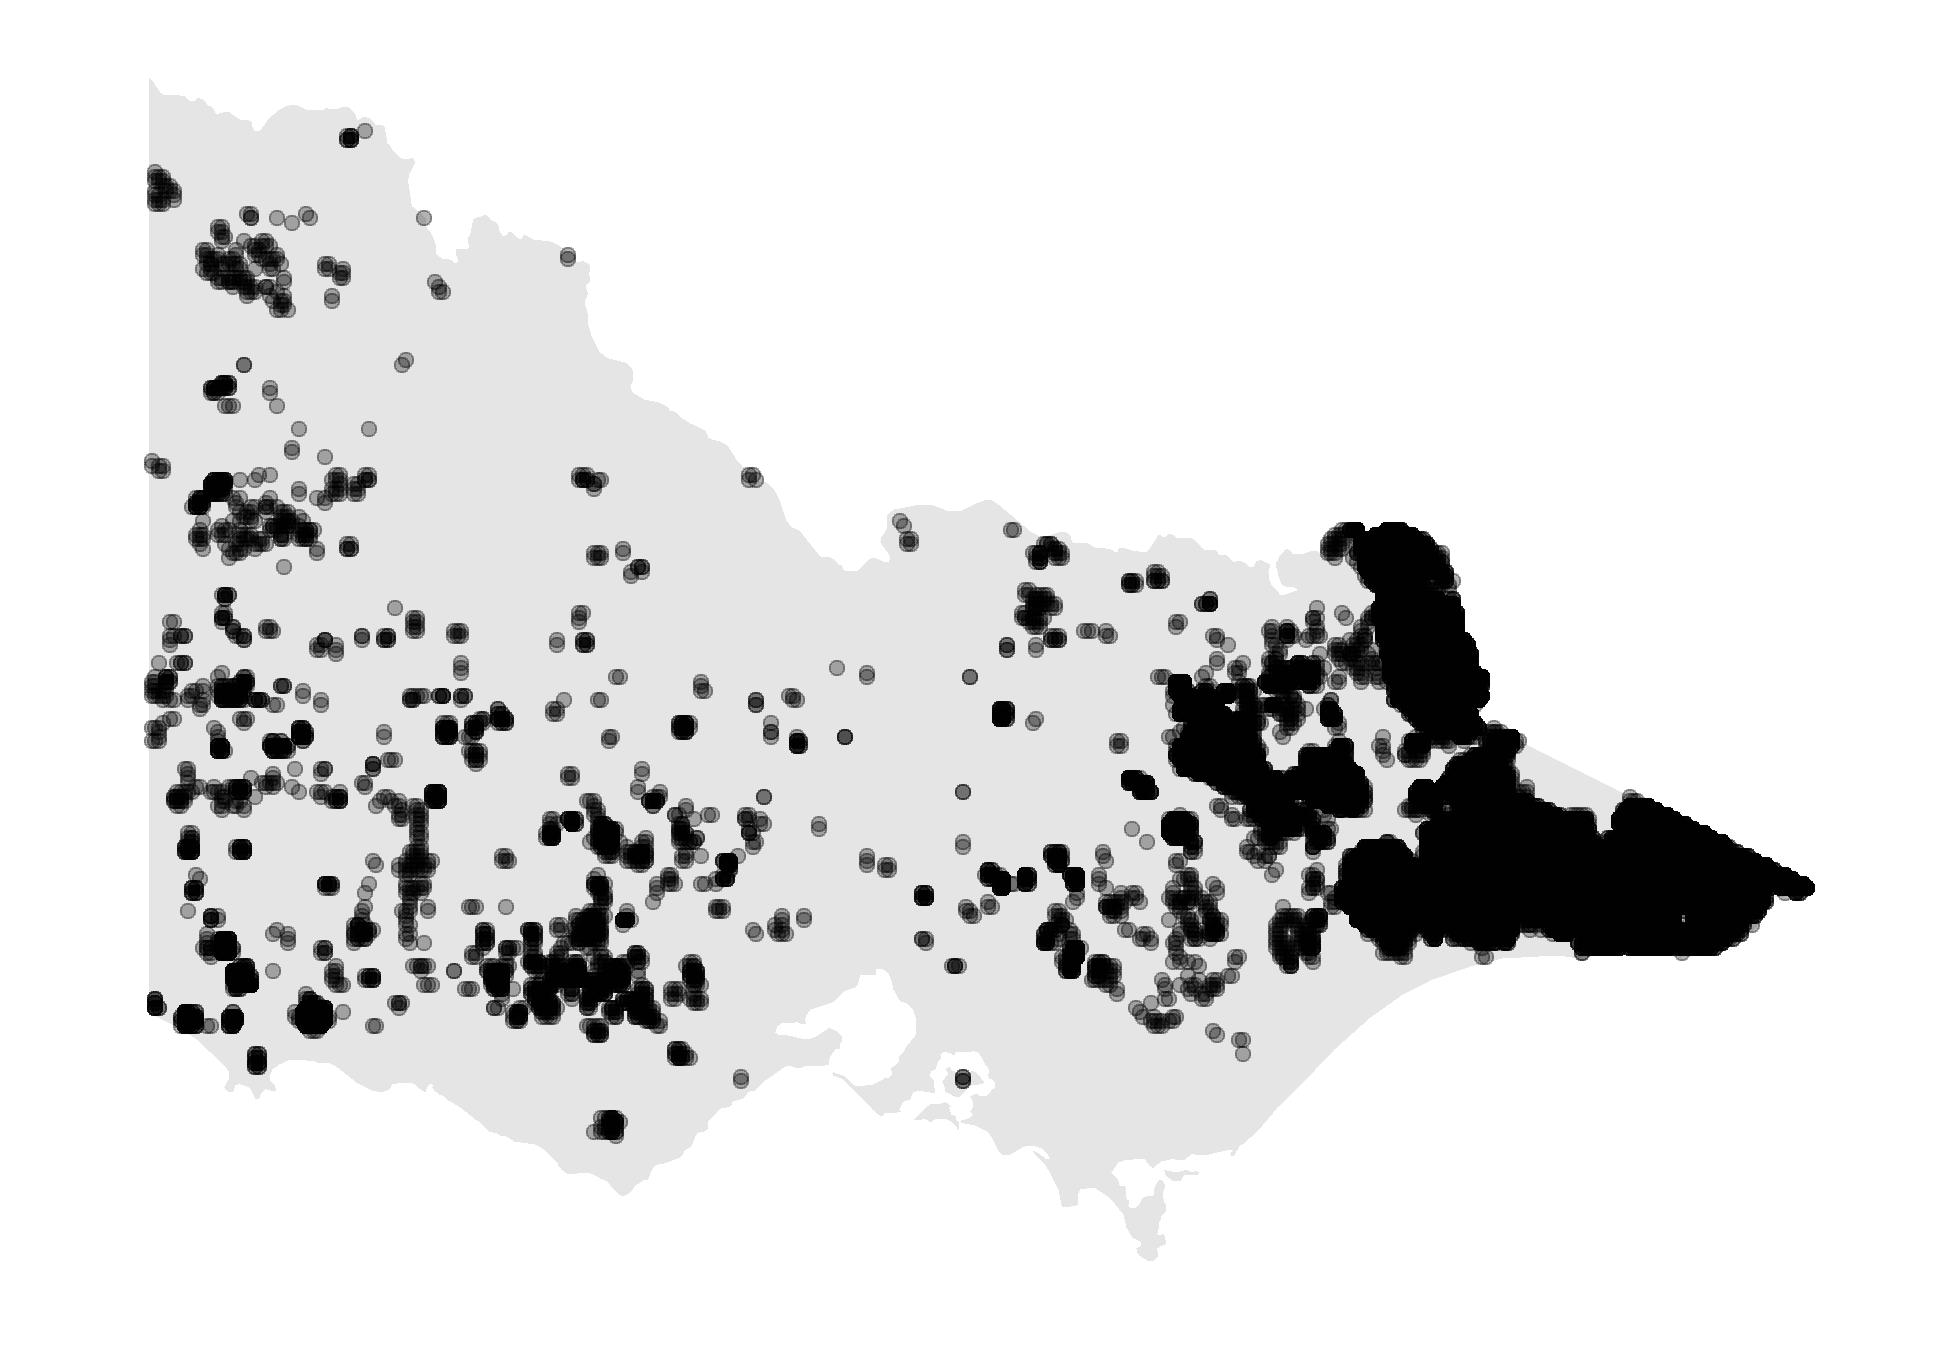
\includegraphics[width=0.8\linewidth]{figures/before_clustering} \caption[A map shown the distribution of hotspot locations in Victoria during 2019-2020 Australia bushfire season]{A map shown the distribution of hotspot locations in Victoria during 2019-2020 Australia bushfire season.}\label{fig:hotspots}
\end{figure}
\end{Schunk}

\hypertarget{steps}{%
\subsubsection{Steps}\label{steps}}

This algorithm was consist of 4 steps:

\begin{enumerate}
\def\labelenumi{\arabic{enumi}.}
\tightlist
\item
  Divided hotspots into different segments
\item
  Clusterd hotspots in each segment individually
\item
  Updated the clustering results recursively
\item
  Computed the ignition location for each cluster
\end{enumerate}

\textbf{1. Divided temporal dimension into different segments}

One of the difficulties to perform clustering on spatiotemporal data was
to determine the scaling of the temporal dimension. Similarly, a
characteristic of hotspot data was cloud cover could lead to missing
observations of a bushfire in several hours. One possible solution for
both issues was flattening the temporal dimension in a small window. In
other words, we predetermined the temporal dependence by introducing a
parameter \(ActiveTime\). The interpretation of \(ActiveTime\) was the
time a fire can stay smouldering but undetectable by satellite before
flaring up again.

Given a certain value of \(ActiveTime\) and the length of the time frame
\(T\), the algorithm would define several segments,

\[\boldsymbol{S}_t = [max(1,t-ActiveTime),t],~~t = 1,2,...,T\]

For example, if the dataset contains 48 hours of hotspots and the
\(ACtiveTime = 24~hours\), there will be 48 segments
\(\boldsymbol{S}_1,\boldsymbol{S}_2,..,\boldsymbol{S}_{48}\), where

\begin{align*}
\boldsymbol{S}_1 &= [1,1]\\
\boldsymbol{S}_2 &= [1,2]\\
&...\\
\boldsymbol{S}_{25} &= [1,25]\\
\boldsymbol{S}_{26} &= [2,26]\\
&...\\
\boldsymbol{S}_{47} &= [23,47]\\
\boldsymbol{S}_{48} &= [24,48]
\end{align*}

\textbf{2. Cluster hotspots in each segment individually}

Since the algorithm broke the temporal dimension in \textbf{step 1}, the
local clustering for each segment only needed to address the hotspots
spatially by introducing the second parameters \(AdjDist\). \(AdjDist\)
represented the potential potential distance a fire could spread with
respect to the temporal resolution of the data. For example, let
\(AdjDist = 3000 m\) and the temporal resolution of the data is
10-minute, then the potential speed of the bushfire is
\(3000m/10~min = 18km/h\).

Given a certain value of \(AdjDist\) and the segment
\(\boldsymbol{S}_t\), the algorithm would

\begin{enumerate}
\def\labelenumi{(\alph{enumi})}
\item
  Append a randomly selected hotspot \(h_i\) to a empty list
  \(\boldsymbol{L}\), where \(h_i\) is the \(i\)th hotspot in the
  segment \(\boldsymbol{S}_t\), and let pointer \(\boldsymbol{P}\) point
  to the first element of the list \(\boldsymbol{L}\).
\item
  Visit every \(h_i\) where \(h_i \notin \boldsymbol{L}\). If
  \(geodesic(h_i, \boldsymbol{P})\leq AdjDist\), append \(h_i\) to list
  \(\boldsymbol{L}\).
\item
  Move pointer \(\boldsymbol{P}\) to the next element of the list
  \(\boldsymbol{L}\).
\item
  Repeat (b) and (c) till the pointer \(\boldsymbol{P}\) reach to the
  end of the list \(\boldsymbol{L}\).
\item
  For hotspots \(h_i \in \boldsymbol{L}\), assign a new membership to
  them. Repeat (a) to (d) for unassigned hotspots in segment
  \(\boldsymbol{S}_t\).
\end{enumerate}

\textbf{3. Updated the clustering results recursively}

\hypertarget{effects-of-parameter-choices}{%
\subsubsection{Effects of parameter
choices}\label{effects-of-parameter-choices}}

There are two parameters that can be tuned in this algorithm. They are
\texttt{adj\_dist}, which is the density distance and
\texttt{active\_time}, which is the .

\hypertarget{application}{%
\subsection{Application}\label{application}}

\hypertarget{determining-the-ignition-point-and-time-for-individual-fires}{%
\subsubsection{Determining the ignition point and time for individual
fires}\label{determining-the-ignition-point-and-time-for-individual-fires}}

Show ignition points for a particularly heavy day and another for a
particularly light day

\begin{Schunk}

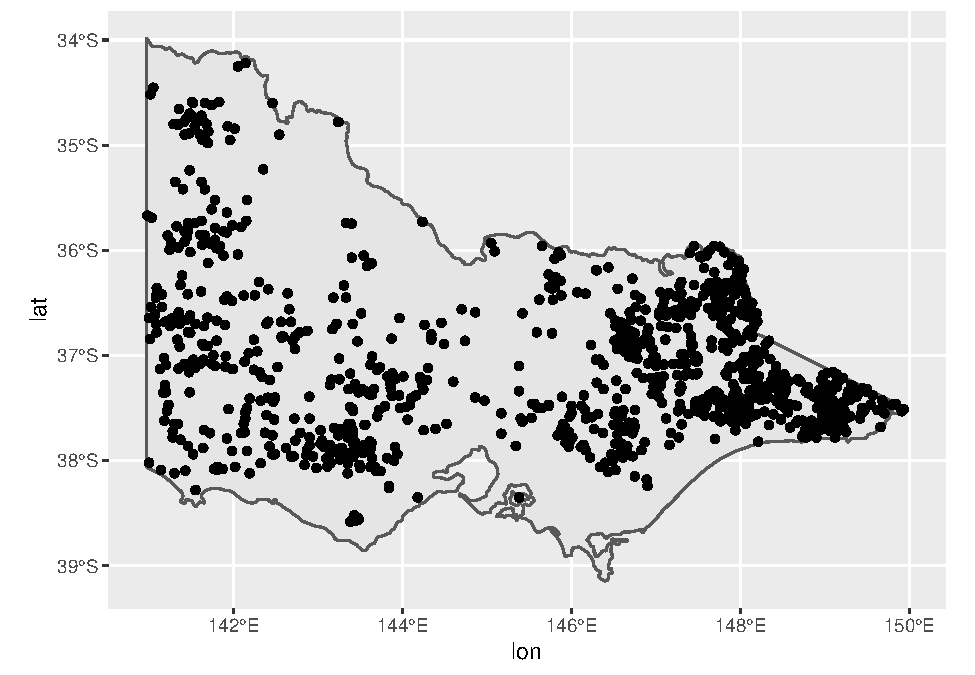
\includegraphics[width=0.8\linewidth]{clustering_paper_files/figure-latex/unnamed-chunk-2-1} \end{Schunk}

\begin{Schunk}

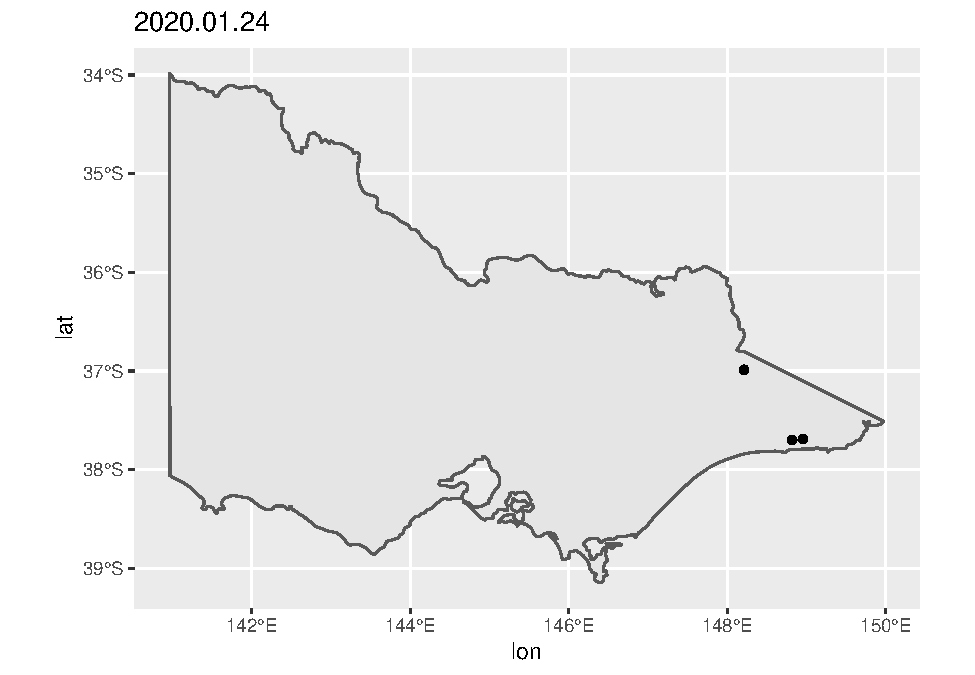
\includegraphics[width=0.8\linewidth]{clustering_paper_files/figure-latex/unnamed-chunk-4-1} \end{Schunk}

\begin{Schunk}

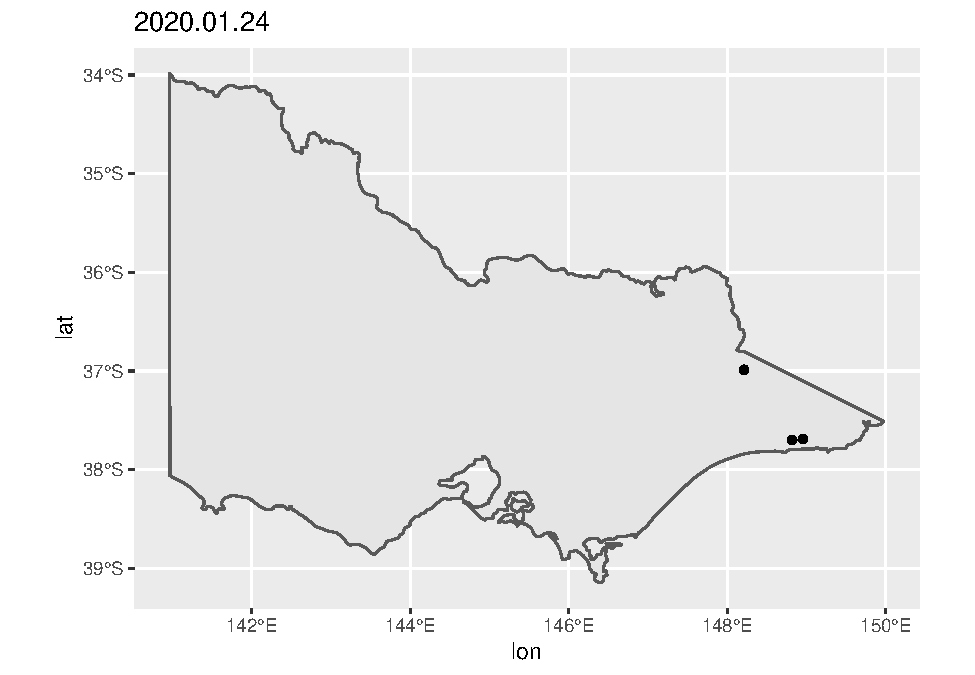
\includegraphics[width=0.8\linewidth]{clustering_paper_files/figure-latex/unnamed-chunk-5-1} \end{Schunk}

\hypertarget{tracking-fire-movement}{%
\subsubsection{Tracking fire movement}\label{tracking-fire-movement}}

Display showing how a fire moves over time, maybe two or more fires

\hypertarget{allocating-resources-for-future-fire-prevention}{%
\subsubsection{Allocating resources for future fire
prevention}\label{allocating-resources-for-future-fire-prevention}}

Merging data with camp sites, CFA, roads, \ldots{}

\hypertarget{summary}{%
\subsection{Summary}\label{summary}}

\hypertarget{acknowledgements}{%
\subsection{Acknowledgements}\label{acknowledgements}}

\begin{itemize}
\tightlist
\item
  The code and files to reproduce this work are at XXX
\item
  Data on hotspots can be downloaded from XXX
\end{itemize}

\bibliography{RJreferences}


\address{%
Weihao Li\\
Monash University\\%
line 1\\ line 2\\
%
%
%
\\\href{mailto:wlii0039@student.monash.edu}{\nolinkurl{wlii0039@student.monash.edu}}
}

\address{%
Emily Dodwell\\
AT\&T\\%
line 1\\ line 2\\
%
%
%
\\\href{mailto:emily@research.att.com}{\nolinkurl{emily@research.att.com}}
}

\address{%
Dianne Cook\\
Monash University\\%
line 1\\ line 2\\
%
%
%
\\\href{mailto:dicook@monash.edu}{\nolinkurl{dicook@monash.edu}}
}

